\documentclass[12pt]{article}
\usepackage{amsmath}
\usepackage{graphicx}
\usepackage{hyperref}
\usepackage[latin1]{inputenc}
\usepackage{listings}
\renewcommand{\labelitemi}{$\textendash$}

\title{CS3031: Project I}
\author{Conor McCauley - 17323203}
\date{February 24, 2020}

\begin{document}

\maketitle

\section{Implementation}

\noindent Upon being started, the web proxy server starts a {\it Tkinter} thread to generate and maintain the graphical user interface (GUI). The server then begins listening to port $8080$ for requests. Whenever a request is received a new thread is created to handle it. This allows the server to handle multiple concurrent requests.

\indent The server reads the raw request data into a {\it ProxyRequest} object which extracts the URL, port, method and other important data from the request. The server ensures that the request is not being sent to a blacklisted URL and then passes the request on to the appropriate handler method: HTTP or HTTPS.

\indent The handler methods relay data between the client and remote server as needed. The HTTPS handler maintains a bidirectional {\it WebSocket} connection. The HTTP handler utilises caching to increase the efficiency of repeated requests.

\subsection{Graphical User Interface}

\noindent The web proxy server uses Python's {\it Tkinter} library to implement the GUI. It allows the user to block or unblock specific URLs while the application is running. It also displays a detailed log of all the requests that were made.

\begin{center}
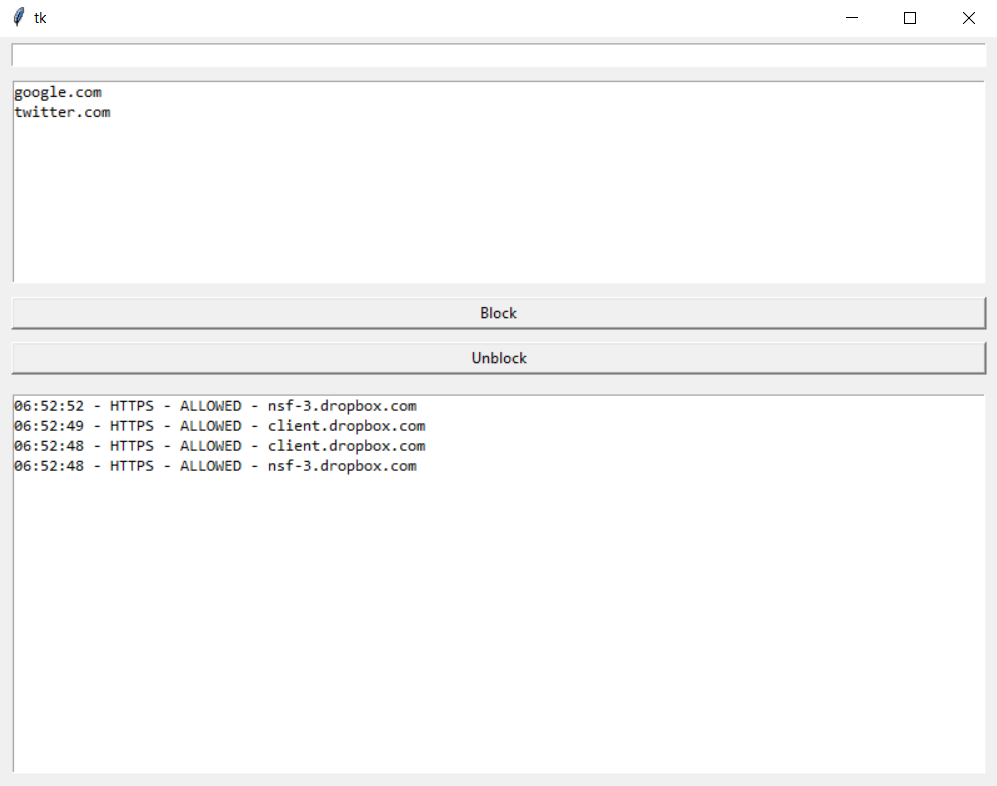
\includegraphics[scale=0.6]{gui.png}
\end{center}

\subsection{URL Blocking}

\noindent Whenever a request is made the destination URL is checked against the user's blacklist - if the URL is contained in the list the request is stopped.

\begin{center}
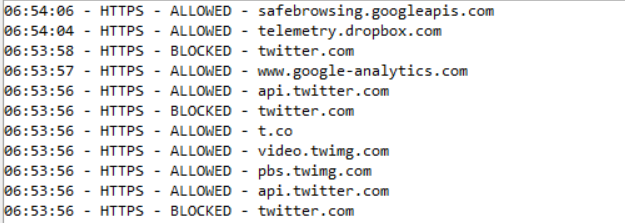
\includegraphics[scale=0.9]{block.png}
\end{center}

\subsection{Response Caching}

\noindent The responses of all HTTP requests are stored in a dictionary and if a subsequent request is made to the same URL the stored response is immediately returned.

\begin{center}
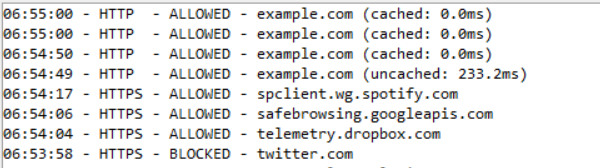
\includegraphics[scale=0.9]{cache.png}
\end{center}

\section{Code Listing}

\lstset{%
    language=Python,
    basicstyle=\small,
    breaklines=true
}
\lstinputlisting{proxy.py}

\end{document}
